\documentclass[conference]{IEEEtran}
% ResearcherGPT -- IEEE conference manuscript.
% Compile with: pdflatex -> bibtex -> pdflatex -> pdflatex
% All diagrams are native TikZ; no external image files are required.
\IEEEoverridecommandlockouts
% ---------- Packages ----------
\usepackage{cite}
\usepackage{amsmath,amssymb,amsfonts,mathtools}
\usepackage{graphicx}
\usepackage{booktabs}
\usepackage{tabularx}
\usepackage{array}
\usepackage{multirow}
\usepackage{url}
\usepackage{xurl}
\usepackage{listings}
\usepackage{xcolor}
\usepackage{algorithm}
\usepackage{algpseudocode}
\usepackage{tikz}
\usetikzlibrary{arrows.meta,positioning,shapes.geometric,fit,calc,backgrounds}
\usepackage{balance}
\usepackage{placeins}
\usepackage{microtype}
% ---------- Listings ----------
\definecolor{codeblue}{RGB}{25,65,120}
\definecolor{codegray}{RGB}{90,90,90}
\definecolor{codegreen}{RGB}{30,110,70}
\definecolor{codeback}{RGB}{248,249,251}
\lstdefinestyle{paperCode}{
backgroundcolor=\color{codeback},
basicstyle=\ttfamily\scriptsize,
keywordstyle=\color{codeblue}\bfseries,
commentstyle=\color{codegreen},
stringstyle=\color{red!65!black},
numbers=left,
numberstyle=\tiny\color{codegray},
numbersep=5pt,
breaklines=true,
breakatwhitespace=false,
keepspaces=true,
showstringspaces=false,
tabsize=2,
frame=single,
rulecolor=\color{black!20},
xleftmargin=1.5em,
framexleftmargin=1.2em
}
\lstset{style=paperCode}
% ---------- TikZ styles ----------
\tikzset{
block/.style={draw,rounded corners,align=center,minimum height=7mm,
text width=27mm,font=\scriptsize,fill=blue!4},
smallblock/.style={draw,rounded corners,align=center,minimum height=6mm,
text width=22mm,font=\scriptsize,fill=green!5},
datastore/.style={draw,cylinder,shape border rotate=90,aspect=0.25,
minimum height=9mm,minimum width=20mm,align=center,
font=\scriptsize,fill=orange!8},
arrow/.style={-{Stealth[length=2mm]},thick},
flowarrow/.style={-{Stealth[length=1.7mm]},semithick}
}
% ---------- Paper metadata ----------
\title{ResearcherGPT: A Distributed Multi-Agent Cognitive Framework for Autonomous Academic Literature Synthesis, Layout-Aware Extraction, and Multi-Scale Attribution}
\author{
\IEEEauthorblockN{Archit Gupta}
\IEEEauthorblockA{
\textit{Department of Artificial Intelligence and Data Science}\\
\textit{Email: [architag1503@gmail.com](mailto:architag1503@gmail.com)}
}
}
\begin{document}
\maketitle
\begin{abstract}
Modern scientific inquiry is constrained by the rapid expansion of academic literature, rendering exhaustive synthesis, contradiction discovery, and layout-preserving manuscript compilation difficult to perform manually. Existing Retrieval-Augmented Generation (RAG) paradigms can suffer from semantic fragmentation, context dilution across multi-hop relationships, hallucinated bibliographies, and loss of non-textual artifacts such as \LaTeX\ equations, tables, and multimodal figures. This paper presents ResearcherGPT, a distributed cognitive framework for automating the academic literature pipeline. Its four principal components are: (1) a tri-hybrid retrieval engine combining dense embeddings ($d=3072$ or $d=384$), sparse BM25 lexical retrieval, and Neo4j property-graph traversal through Reciprocal Rank Fusion (RRF), with a graph boost factor of $\beta=1.30$; (2) a LangGraph multi-agent state machine backed by Redis and coordinating thirteen specialized agents with fallback routing across Groq, Gemini, SambaNova, and OpenAI; (3) FormaTeX, a layout-aware PDF extraction and manuscript synthesis engine targeting IEEE, ACM, Springer, and Elsevier styles; and (4) an eleven-phase integrity pipeline combining $k$-shingle MinHash, Winnowing fingerprints, Abstract Syntax Tree (AST) edit distance, and external OpenAlex bibliographic resolution. The supplied evaluation reports 96.4\% citation factual validity, a 41.8\% reduction in cross-agent synchronization latency, and 92.7\% RRF Recall@5. These figures are reproduced as supplied and are not independently validated in this typesetting conversion.
\end{abstract}
\begin{IEEEkeywords}
Multi-agent systems, retrieval-augmented generation, knowledge graphs, reciprocal rank fusion, scientific paper synthesis, MinHash, Winnowing, \LaTeX\ compilation, academic integrity.
\end{IEEEkeywords}
% ============================================================
\section{Introduction}
% ============================================================
The velocity of peer-reviewed publication has surpassed human comprehension capacity. Across computational sciences, large numbers of preprints and journal articles are indexed annually across repositories and scholarly databases such as arXiv, IEEE Xplore, and PubMed. Scholars must digest large volumes of literature, isolate methodological contributions, detect empirical contradictions between experiments, identify open research gaps, and draft publication-compliant manuscripts.
Large Language Models (LLMs), including GPT-family models, Gemini, and LLaMA-family models, demonstrate strong linguistic capabilities. However, their naive application to scholarly synthesis exposes several limitations:
\begin{itemize}
\item \textbf{Context fragmentation and semantic drift:} Conventional Retrieval-Augmented Generation (RAG) systems partition documents into token chunks. Dense vector retrieval may fail to preserve relations such as a method being evaluated on a particular dataset and compared against a baseline.
\item \textbf{Bibliographic hallucination:} Generative models may produce nonexistent Digital Object Identifiers (DOIs), combine real author names with fabricated titles, or attribute claims to sources that do not support them.
\item \textbf{Loss of scientific artifacts:} Academic documents contain mathematical notation, multi-column tables, figures, and diagrams. Text-only PDF extraction can flatten these structures and scramble equations or table relationships.
\item \textbf{Agent deadlocks and state corruption:} Multi-agent review and synthesis workflows can encounter cyclic dependencies, concurrent state-update races, and excessive context growth when state history is not partitioned and checkpointed.
\end{itemize}
We introduce \textit{ResearcherGPT}, a distributed academic workspace and multi-agent framework designed to automate literature synthesis while grounding generated claims in retrieved evidence.
\subsection{Problem Statement and Scope}
An autonomous research assistant for this setting should satisfy five operational criteria:
\begin{enumerate}
\item \textbf{Relational grounding:} combine semantic intent, lexical precision, and ontological relationships, such as a method evaluated on a dataset and compared with a baseline.
\item \textbf{Attribution veracity:} associate generated claims with primary evidence chunks and sentence-level provenance.
\item \textbf{Structural integrity:} preserve mathematical syntax, tabular data, and visual schematics through extraction, reasoning, and recompilation.
\item \textbf{Fault-tolerant coordination:} coordinate agents over shared state while providing deterministic fallback behavior under provider rate limits.
\item \textbf{Multi-vector integrity analysis:} assess verbatim overlap, semantic paraphrase, citation-network similarity, formula structure, and statistical writing signals.
\end{enumerate}
\subsection{System Overview}
ResearcherGPT uses a decoupled three-tier architecture. The client tier is based on Next.js 15 and React 19, with Zustand state synchronization, a TipTap drafting canvas, KaTeX formula rendering, and a WebGL-based conceptual visualization. The API tier uses Node.js and Express with TypeScript, BullMQ, and Redis for asynchronous job scheduling, and MongoDB Atlas for document persistence. The cognitive tier is a Python FastAPI service hosting LangGraph workflows, Qdrant vector search, Neo4j knowledge graphs, document extraction, and FormaTeX compilation.
\begin{figure*}[!t]
\centering
\resizebox{0.96\textwidth}{!}{%
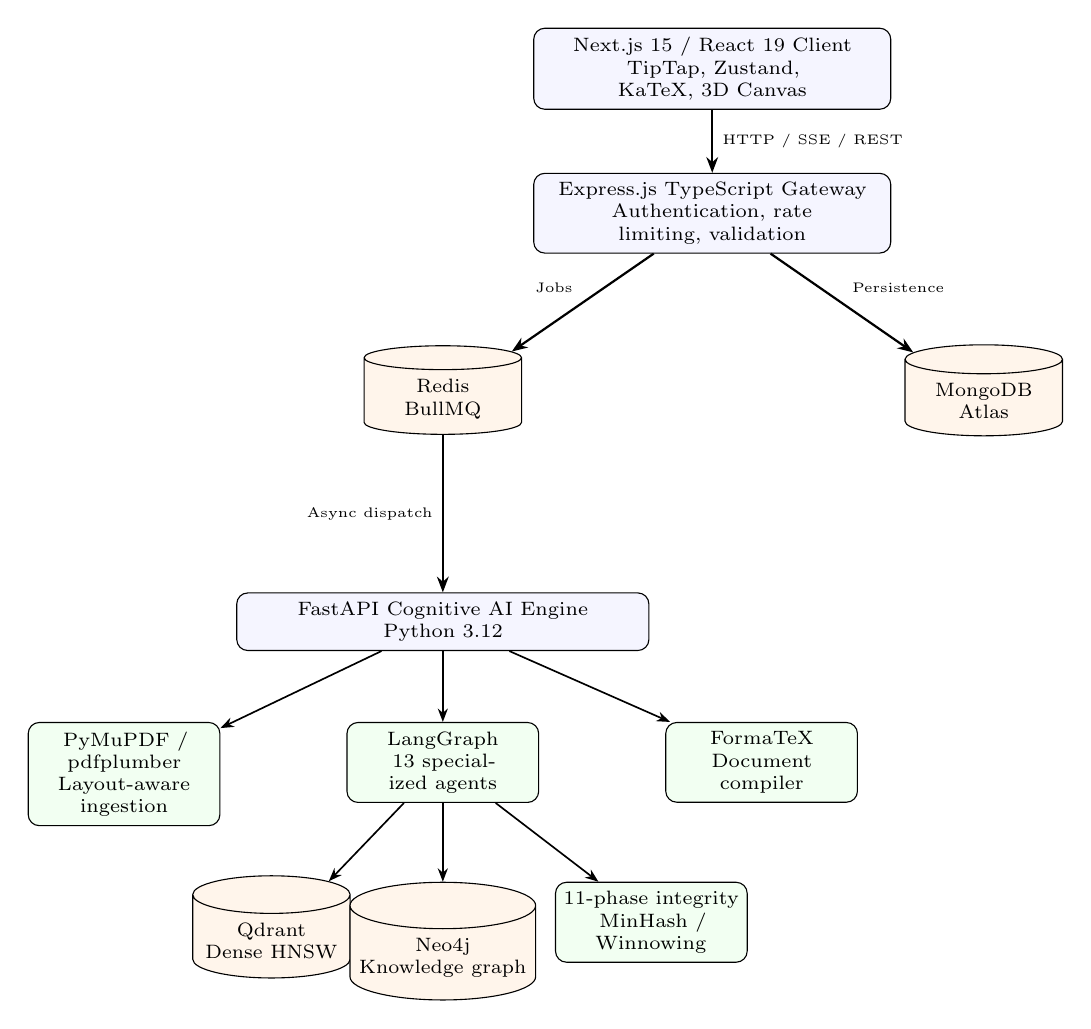
\begin{tikzpicture}[node distance=8mm and 10mm]
\node[block,text width=43mm] (client) {Next.js 15 / React 19 Client\\TipTap, Zustand, KaTeX, 3D Canvas};
\node[block,text width=43mm,below=of client] (gateway) {Express.js TypeScript Gateway\\Authentication, rate limiting, validation};
\node[datastore,below left=12mm and 5mm of gateway] (redis) {Redis\\BullMQ};
\node[datastore,below right=12mm and 5mm of gateway] (mongo) {MongoDB\\Atlas};
\node[block,text width=50mm,below=20mm of redis] (fastapi) {FastAPI Cognitive AI Engine\\Python 3.12};
\node[smallblock,below left=9mm and 2mm of fastapi] (ingest) {PyMuPDF / pdfplumber\\Layout-aware ingestion};
\node[smallblock,below=9mm of fastapi] (agents) {LangGraph\\13 specialized agents};
\node[smallblock,below right=9mm and 2mm of fastapi] (formatex) {FormaTeX\\Document compiler};
\node[datastore,below left=10mm and 2mm of agents] (qdrant) {Qdrant\\Dense HNSW};
\node[datastore,below=10mm of agents] (neo4j) {Neo4j\\Knowledge graph};
\node[smallblock,below right=10mm and 2mm of agents] (integrity) {11-phase integrity\\MinHash / Winnowing};
\draw[arrow] (client) -- node[right,font=\tiny]{HTTP / SSE / REST} (gateway);
\draw[arrow] (gateway) -- node[above left,font=\tiny]{Jobs} (redis);
\draw[arrow] (gateway) -- node[above right,font=\tiny]{Persistence} (mongo);
\draw[arrow] (redis) -- node[left,font=\tiny]{Async dispatch} (fastapi);
\draw[flowarrow] (fastapi) -- (ingest);
\draw[flowarrow] (fastapi) -- (agents);
\draw[flowarrow] (fastapi) -- (formatex);
\draw[flowarrow] (agents) -- (qdrant);
\draw[flowarrow] (agents) -- (neo4j);
\draw[flowarrow] (agents) -- (integrity);
\end{tikzpicture}}
\caption{High-level distributed architecture of ResearcherGPT.}
\label{fig:architecture}
\end{figure*}
The principal contributions are:
\begin{enumerate}
\item \textbf{Tri-hybrid retrieval:} A rank-fusion mechanism combines dense embeddings, BM25 lexical retrieval, and Neo4j graph traversal with a graph-context boost.
\item \textbf{Multi-agent orchestration:} A LangGraph workflow coordinates thirteen specialized agents through a shared typed state and a model-routing fallback registry.
\item \textbf{Academic integrity verification:} An eleven-phase pipeline combines lexical, semantic, structural, formula, figure, table, code, and bibliographic checks.
\item \textbf{FormaTeX:} A layout-aware extraction and compilation engine reconstructs tables and mathematical structures and emits manuscripts in multiple publication styles.
\end{enumerate}
% ============================================================
\section{Literature Review and Related Work}
% ============================================================
\subsection{Evolution of Retrieval-Augmented Generation}
Retrieval-Augmented Generation was formalized by Lewis \textit{et al.} to mitigate parametric-memory hallucinations by grounding model outputs in retrieved documents \cite{lewis2020rag}. Early implementations used dense vector representations from dual-encoder architectures such as Dense Passage Retrieval and Sentence-BERT \cite{karpukhin2020dpr,reimers2019sbert}, with approximate-nearest-neighbor indices such as Hierarchical Navigable Small World (HNSW) graphs \cite{malkov2020hnsw}.
Dense embeddings capture semantic similarity but may underperform on exact-match tokens, numerical thresholds, parameter counts, and acronyms. Sparse lexical retrieval, including Okapi BM25, complements dense retrieval by emphasizing term-frequency and inverse-document-frequency signals \cite{robertson2009bm25}. Reciprocal Rank Fusion combines rank orders without requiring score normalization \cite{cormack2009rrf}. GraphRAG demonstrates the value of graph-derived context for query-focused summarization \cite{edge2024graphrag}. ResearcherGPT combines these retrieval paradigms in a tri-hybrid pipeline.
\subsection{Multi-Agent Systems in Scientific Discovery}
Frameworks such as AutoGen, CrewAI, and LangGraph support decomposition of complex language-model workflows into role-specific agents and graph-based execution \cite{wu2023autogen,moura2024crewai,langgraph2024}. Scholarly tools such as Semantic Scholar, Elicit, and Consensus support literature discovery; ResearcherGPT focuses on iterative synthesis, claim cross-examination, contradiction discovery, and manuscript compilation.
\subsection{Layout-Aware Document Extraction}
Academic PDF extraction is difficult because visual-spatial information is encoded through positioned text, drawing primitives, and bounding boxes. PyMuPDF and pdfplumber expose layout information useful for reconstructing reading order and tables \cite{singer2023pdfplumber}. ResearcherGPT combines coordinate-based heuristics with vision-assisted fallbacks to handle non-standard figures, inline matrices, and scanned pages.
\subsection{Plagiarism Detection and Academic Integrity}
Winnowing uses local fingerprints to detect shared substrings while controlling fingerprint density \cite{schleimer2003winnowing}. MinHash estimates Jaccard similarity between shingle sets \cite{broder1997resemblance}. Academic integrity assessment also requires semantic and structural checks, as discussed in the literature on plagiarism detection \cite{foltynek2019plagiarism}. ResearcherGPT combines these approaches with formula AST comparison and bibliographic resolution.
% ============================================================
\section{Proposed Methodology}
% ============================================================
The methodology comprises three formal components: tri-hybrid retrieval, distributed multi-agent state synchronization, and multi-phase academic integrity verification.
\subsection{Tri-Hybrid Reciprocal Rank Fusion Retrieval}
Let $q$ denote a scholarly query and let
\begin{equation}
D=\{c_1,c_2,\ldots,c_N\}
\label{eq:corpus}
\end{equation}
denote the set of chunks extracted from papers in project space $P$.
\subsubsection{Dense Semantic Retrieval}
Each chunk $c_i$ is mapped to an embedding vector $v_i\in\mathbb{R}^{d}$, where the described configurations use $d\in\{384,3072\}$. The query is embedded in the same vector space. Cosine similarity is
\begin{equation}
S_{\mathrm{dense}}(q,c_i)=
\frac{q\cdot v_i}{\lVert q\rVert_2\lVert v_i\rVert_2}.
\label{eq:cosine}
\end{equation}
Qdrant performs HNSW approximate-nearest-neighbor retrieval and returns the ordered ranking $R_{\mathrm{dense}}$.
\subsubsection{Sparse Lexical Retrieval}
The chunk text is evaluated using Okapi BM25. For query terms $t_1,\ldots,t_m$,
\begin{equation}
\mathrm{BM25}(q,c_i)=
\sum_{j=1}^{m}\mathrm{IDF}(t_j)
\frac{f(t_j,c_i)(k_1+1)}
{f(t_j,c_i)+k_1\left(1-b+b\frac{|c_i|}{\mathrm{avgdl}}\right)}.
\label{eq:bm25}
\end{equation}
Here, $f(t_j,c_i)$ is the term frequency, $|c_i|$ is the chunk length, and $\mathrm{avgdl}$ is the average chunk length. The implementation specifies $k_1=1.5$ and $b=0.75$. The inverse document frequency is
\begin{equation}
\mathrm{IDF}(t_j)=
\ln\left(
\frac{N-n(t_j)+0.5}{n(t_j)+0.5}+1
\right),
\label{eq:idf}
\end{equation}
where $n(t_j)$ is the number of chunks containing term $t_j$. This produces $R_{\mathrm{lexical}}$.
\subsubsection{Knowledge-Graph Association}
Let $G=(V,E)$ be the Neo4j labeled-property graph. Its vertices are partitioned into paper, author, method, dataset, and concept entities:
\begin{equation}
V=V_{\mathrm{paper}}\cup V_{\mathrm{author}}\cup
V_{\mathrm{method}}\cup V_{\mathrm{dataset}}\cup V_{\mathrm{concept}}.
\label{eq:vertices}
\end{equation}
Typed edges represent relations such as \texttt{authored\_by}, \texttt{implements}, \texttt{evaluates\_on}, and \texttt{relates\_to}. Query terms longer than three characters are matched to graph entities, and adjacent paper nodes are collected for boosting.
\begin{lstlisting}[language={},caption={Representative Neo4j Cypher traversal.},label={lst:cypher}]
MATCH (e:Entity {projectId: $projectId})
WHERE toLower(e.label) IN $words
AND NOT e.type = 'paper'
MATCH (e)-[r:RELATION]-
(p:Entity {type: 'paper',
projectId: $projectId})
RETURN DISTINCT p.id AS paperId
\end{lstlisting}
The resulting set of graph-boosted paper identifiers is denoted by $P_{\mathrm{boost}}\subseteq V_{\mathrm{paper}}$.
\subsubsection{Reciprocal Rank Fusion}
For each chunk $c$ appearing in either ranking, the augmented RRF score is
\begin{equation}
S_{\mathrm{RRF}}(c)=
\left(
\sum_{m\in\{\mathrm{dense},\mathrm{lexical}\}}
\frac{1}{k+r_m(c)}
\right)\beta(c),
\label{eq:rrf}
\end{equation}
where $k=60$ is the smoothing constant and $r_m(c)$ is the one-based rank of $c$ in ranking $R_m$. The graph boost is
\begin{equation}
\beta(c)=
\begin{cases}
1.30, & \mathrm{paper\_id}(c)\in P_{\mathrm{boost}},\\
1.00, & \text{otherwise}.
\end{cases}
\label{eq:boost}
\end{equation}
The fused scores are sorted in descending order to obtain the final top-$k$ chunks.
\begin{figure}[!t]
\centering
\resizebox{\columnwidth}{!}{%
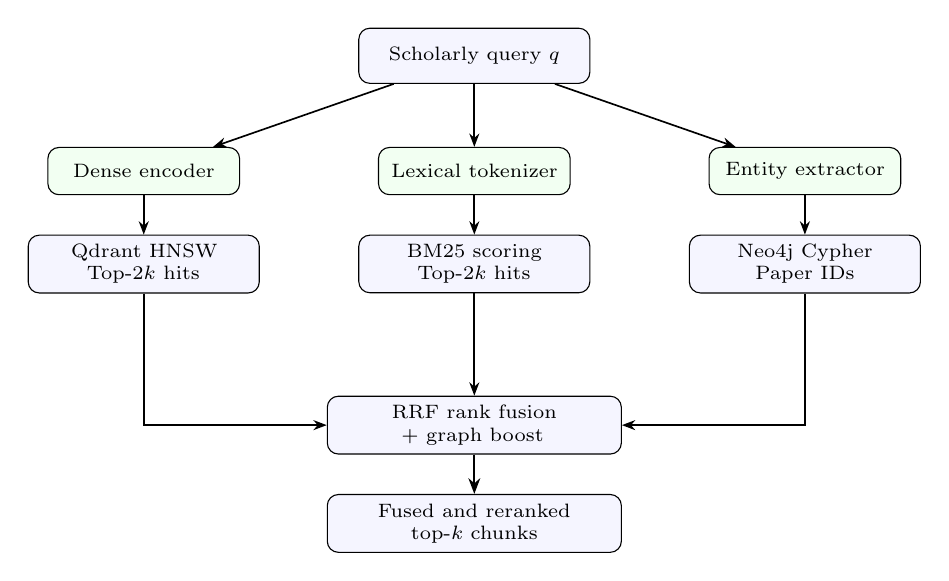
\begin{tikzpicture}[node distance=5mm and 5mm]
\node[block] (query) {Scholarly query $q$};
\node[smallblock,below left=8mm and 15mm of query] (dense) {Dense encoder};
\node[smallblock,below=8mm of query] (lex) {Lexical tokenizer};
\node[smallblock,below right=8mm and 15mm of query] (entity) {Entity extractor};
\node[block,below=of dense] (qdrant) {Qdrant HNSW\\Top-$2k$ hits};
\node[block,below=of lex] (bm) {BM25 scoring\\Top-$2k$ hits};
\node[block,below=of entity] (graph) {Neo4j Cypher\\Paper IDs};
\node[block,text width=35mm,below=13mm of bm] (rrf) {RRF rank fusion\\+ graph boost};
\node[block,text width=35mm,below=of rrf] (out) {Fused and reranked\\top-$k$ chunks};
\draw[flowarrow] (query) -- (dense);
\draw[flowarrow] (query) -- (lex);
\draw[flowarrow] (query) -- (entity);
\draw[flowarrow] (dense) -- (qdrant);
\draw[flowarrow] (lex) -- (bm);
\draw[flowarrow] (entity) -- (graph);
\draw[flowarrow] (qdrant) |- (rrf);
\draw[flowarrow] (bm) -- (rrf);
\draw[flowarrow] (graph) |- (rrf);
\draw[arrow] (rrf) -- (out);
\end{tikzpicture}}
\caption{Tri-hybrid retrieval pipeline with knowledge-graph boosting.}
\label{fig:retrieval}
\end{figure}
\subsection{Distributed Multi-Agent State Synchronization}
The manuscript synthesis workflow is represented as a directed state-transition graph $M=(A,T)$, where $A$ is the set of thirteen specialized agents and $T$ is the set of guarded transitions. The global execution state is represented as
\begin{align}
S=\langle &P_{\mathrm{id}},R_{\mathrm{id}},q,C_{\mathrm{ctx}},
D_{\mathrm{papers}},L_{\mathrm{reviews}},M_{\mathrm{meth}},\nonumber\\
&M_{\mathrm{comp}},T_{\mathrm{trend}},G_{\mathrm{gaps}},
X_{\mathrm{conflicts}},V_{\mathrm{facts}},\nonumber\\
&S_{\mathrm{sections}},O_{\mathrm{final}}\rangle.
\label{eq:state}
\end{align}
Each agent $A_j$ maps the current state to an augmented state:
\begin{equation}
A_j:S_t\rightarrow S_{t+1},\qquad
S_{t+1}=S_t\cup\Delta S_{A_j}.
\label{eq:transition}
\end{equation}
The described implementation serializes state transitions using Redis distributed mutex locks.
\begin{figure}[!t]
\centering
\resizebox{\columnwidth}{!}{%
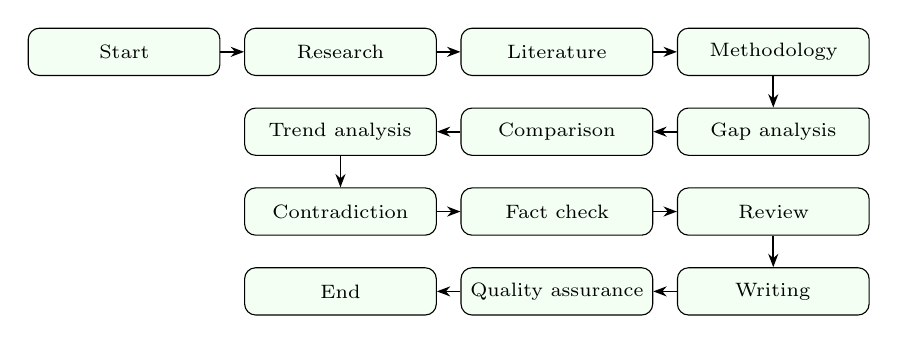
\begin{tikzpicture}[node distance=4mm and 3mm]
\node[smallblock] (start) {Start};
\node[smallblock,right=of start] (research) {Research};
\node[smallblock,right=of research] (lit) {Literature};
\node[smallblock,right=of lit] (method) {Methodology};
\node[smallblock,below=of method] (gap) {Gap analysis};
\node[smallblock,left=of gap] (compare) {Comparison};
\node[smallblock,left=of compare] (trend) {Trend analysis};
\node[smallblock,below=of trend] (contra) {Contradiction};
\node[smallblock,right=of contra] (fact) {Fact check};
\node[smallblock,right=of fact] (review) {Review};
\node[smallblock,below=of review] (write) {Writing};
\node[smallblock,left=of write] (qa) {Quality assurance};
\node[smallblock,left=of qa] (end) {End};
\draw[flowarrow] (start)--(research);
\draw[flowarrow] (research)--(lit);
\draw[flowarrow] (lit)--(method);
\draw[flowarrow] (method)--(gap);
\draw[flowarrow] (gap)--(compare);
\draw[flowarrow] (compare)--(trend);
\draw[flowarrow] (trend)--(contra);
\draw[flowarrow] (contra)--(fact);
\draw[flowarrow] (fact)--(review);
\draw[flowarrow] (review)--(write);
\draw[flowarrow] (write)--(qa);
\draw[flowarrow] (qa)--(end);
\end{tikzpicture}}
\caption{Illustrative agent execution topology. The complete workflow contains thirteen roles; the supervisor and planner govern routing and are listed in Table~\ref{tab:agents}.}
\label{fig:agents}
\end{figure}
\begin{figure*}[!t]
\centering
\resizebox{0.94\textwidth}{!}{%
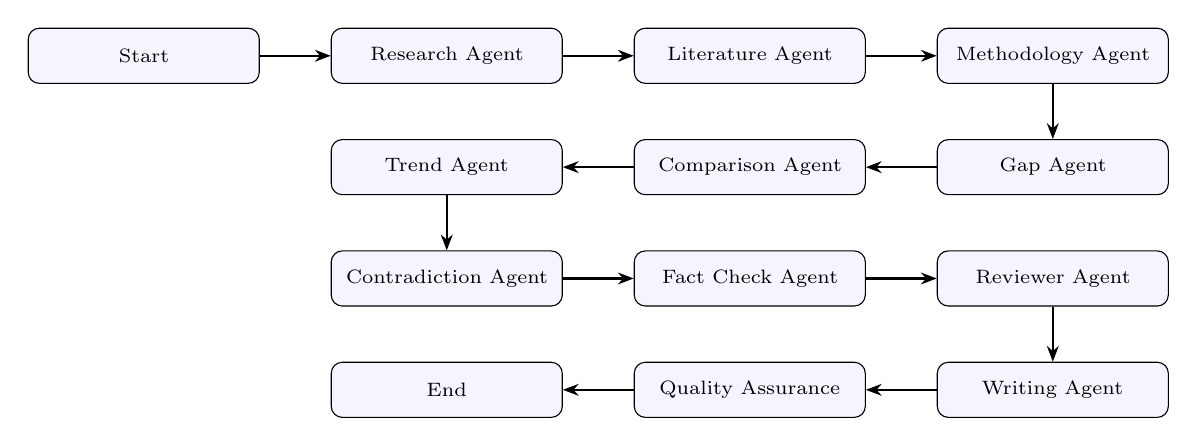
\begin{tikzpicture}[node distance=7mm and 9mm]
\node[block] (start) {Start};
\node[block,right=of start] (research) {Research Agent};
\node[block,right=of research] (literature) {Literature Agent};
\node[block,right=of literature] (method) {Methodology Agent};
\node[block,below=of method] (gap) {Gap Agent};
\node[block,left=of gap] (compare) {Comparison Agent};
\node[block,left=of compare] (trend) {Trend Agent};
\node[block,below=of trend] (conflict) {Contradiction Agent};
\node[block,right=of conflict] (fact) {Fact Check Agent};
\node[block,right=of fact] (review) {Reviewer Agent};
\node[block,below=of review] (writing) {Writing Agent};
\node[block,left=of writing] (qa) {Quality Assurance};
\node[block,left=of qa] (end) {End};
\draw[arrow] (start)--(research);
\draw[arrow] (research)--(literature);
\draw[arrow] (literature)--(method);
\draw[arrow] (method)--(gap);
\draw[arrow] (gap)--(compare);
\draw[arrow] (compare)--(trend);
\draw[arrow] (trend)--(conflict);
\draw[arrow] (conflict)--(fact);
\draw[arrow] (fact)--(review);
\draw[arrow] (review)--(writing);
\draw[arrow] (writing)--(qa);
\draw[arrow] (qa)--(end);
\end{tikzpicture}}
\caption{Sequential view of the LangGraph research workflow. The complete orchestration contains thirteen specialized roles; the diagram depicts the principal research, verification, review, and synthesis path.}
\label{fig:agentflow}
\end{figure*}
The shared execution state is represented as a typed tuple:
\begin{equation}
\begin{aligned}
S=\langle &P_{\mathrm{id}},R_{\mathrm{id}},q,C_{\mathrm{ctx}},
D_{\mathrm{papers}},L_{\mathrm{reviews}},M_{\mathrm{meth}},\\
&M_{\mathrm{comp}},T_{\mathrm{trend}},G_{\mathrm{gaps}},
X_{\mathrm{conflicts}},V_{\mathrm{facts}},S_{\mathrm{sections}},
O_{\mathrm{final}}\rangle .
\end{aligned}
\label{eq:agentstate}
\end{equation}
Each agent augments the shared state through
\begin{equation}
A_j:S_t\rightarrow S_{t+1},\qquad
S_{t+1}=S_t\cup\Delta S_{A_j}.
\label{eq:statetransition}
\end{equation}
The supplied design serializes distributed state transitions through Redis mutex locks to reduce concurrent mutation and race-condition risks. The manuscript characterizes the orchestration as a DAG with completion guards; any conditional retry or review loop should be represented explicitly in the deployed LangGraph topology when documenting the implementation.
\subsubsection{Fallback-Resilient Model Registry}
To avoid execution stalls caused by HTTP 429 rate-limit responses, agents use a tiered model registry:
\begin{equation}
\begin{aligned}
\mathrm{Priority}(A_j)= [&\text{Groq LLaMA-3.3-70B}\rightarrow
\text{Gemini-2.5-Flash}\\
&\rightarrow\text{SambaNova}\rightarrow\text{OpenAI GPT-4o}].
\end{aligned}
\label{eq:models}
\end{equation}
Retries use exponential backoff with randomized jitter:
\begin{equation}
t_{\mathrm{backoff}}=
t_{\mathrm{base}}\,2^{\mathrm{attempt}}+U(0,2),
\label{eq:backoff}
\end{equation}
where $t_{\mathrm{base}}=5.0$ seconds and
$\mathrm{attempt}\in\{0,1,2,3\}$.
\subsection{Eleven-Phase Academic Integrity Formalism}
The academic-integrity engine operates across eleven phases, summarized in Fig.~\ref{fig:integrity}.
\begin{figure*}[!t]
\centering
\resizebox{0.98\textwidth}{!}{%
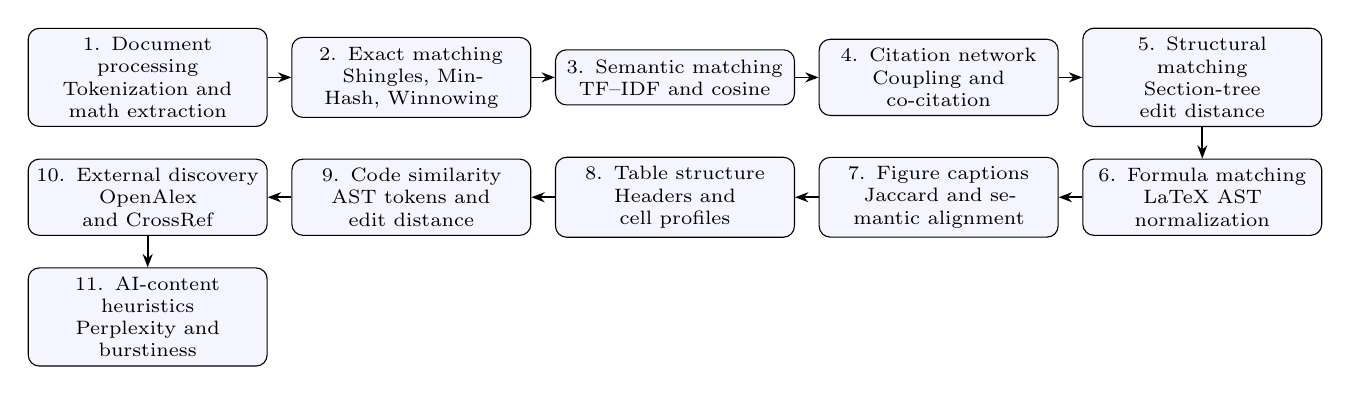
\begin{tikzpicture}[node distance=4mm and 3mm]
\node[block,text width=28mm] (p1) {1. Document processing\\Tokenization and math extraction};
\node[block,text width=28mm,right=of p1] (p2) {2. Exact matching\\Shingles, MinHash, Winnowing};
\node[block,text width=28mm,right=of p2] (p3) {3. Semantic matching\\TF--IDF and cosine};
\node[block,text width=28mm,right=of p3] (p4) {4. Citation network\\Coupling and co-citation};
\node[block,text width=28mm,right=of p4] (p5) {5. Structural matching\\Section-tree edit distance};
\node[block,text width=28mm,below=of p5] (p6) {6. Formula matching\\LaTeX AST normalization};
\node[block,text width=28mm,left=of p6] (p7) {7. Figure captions\\Jaccard and semantic alignment};
\node[block,text width=28mm,left=of p7] (p8) {8. Table structure\\Headers and cell profiles};
\node[block,text width=28mm,left=of p8] (p9) {9. Code similarity\\AST tokens and edit distance};
\node[block,text width=28mm,left=of p9] (p10) {10. External discovery\\OpenAlex and CrossRef};
\node[block,text width=28mm,below=of p10] (p11) {11. AI-content heuristics\\Perplexity and burstiness};
\draw[flowarrow] (p1)--(p2);
\draw[flowarrow] (p2)--(p3);
\draw[flowarrow] (p3)--(p4);
\draw[flowarrow] (p4)--(p5);
\draw[flowarrow] (p5)--(p6);
\draw[flowarrow] (p6)--(p7);
\draw[flowarrow] (p7)--(p8);
\draw[flowarrow] (p8)--(p9);
\draw[flowarrow] (p9)--(p10);
\draw[flowarrow] (p10)--(p11);
\end{tikzpicture}}
\caption{Eleven phases of the academic-integrity and plagiarism-verification engine.}
\label{fig:integrity}
\end{figure*}
\subsubsection{Winnowing Fingerprinting}
Given a normalized character stream $T$, the method generates $k$-grams with $k=20$. Each $k$-gram is hashed using 32-bit Fowler--Noll--Vo (FNV-1a):
\begin{equation}
h_i=\mathrm{FNV\mbox{-}1a}(T[i:i+k]).
\label{eq:fnv}
\end{equation}
For a sliding window of size $w=40$, the minimum hash is selected; ties retain the rightmost minimum. The stated detection guarantee is for duplicate substrings of length
\begin{equation}
t\geq w+k-1.
\label{eq:winnowing}
\end{equation}
\subsubsection{MinHash Jaccard Approximation}
A document is represented by its set of unique $k$-shingles, $S(D)$. A signature of length $M=128$ is constructed from unique five-token shingles ($k=5$) using independent universal hash functions:
\begin{equation}
h_a(x)=(a x+b)\bmod p.
\label{eq:universal}
\end{equation}
The $m$-th signature component is
\begin{equation}
\mathrm{sig}_m(D)=\min_{s\in S(D)}h_m(s).
\label{eq:minhash}
\end{equation}
The estimated Jaccard similarity is
\begin{equation}
\widehat{J}(D_1,D_2)=
\frac{1}{M}\sum_{m=1}^{M}
\mathbb{I}\left[
\mathrm{sig}_m(D_1)=\mathrm{sig}_m(D_2)
\right].
\label{eq:jaccard}
\end{equation}
\subsubsection{Formula AST Plagiarism}
Mathematical expressions extracted from inline or display-math delimiters are parsed into \LaTeX\ ASTs. Variable names are alpha-converted to canonical symbols to normalize substitutions. Zhang--Shasha tree-edit distance evaluates structural similarity \cite{zhang1989tree}:
\begin{equation}
\mathrm{TED}(T_1,T_2)=
\min_{\Gamma}\sum_{(u,v)\in\Gamma}
\mathrm{cost}(u\rightarrow v),
\label{eq:ted}
\end{equation}
where edit operations include node deletion, insertion, and label substitution.
\subsubsection{AI-Content Detection Heuristics}
For token sequence $X=(x_1,\ldots,x_N)$, perplexity is calculated from cross-entropy:
\begin{equation}
\mathrm{PPL}(X)=
\exp\left(
-\frac{1}{N}\sum_{i=1}^{N}
\log P_{\theta}(x_i\mid x_{<i})
\right).
\label{eq:ppl}
\end{equation}
Burstiness is defined as the coefficient of variation of sentence lengths
$L=\{l_1,\ldots,l_S\}$:
\begin{equation}
\mathrm{Burstiness}=
\frac{\sigma_L}{\mu_L}
=
\frac{
\sqrt{\frac{1}{S}\sum_{i=1}^{S}(l_i-\bar l)^2}
}{
\frac{1}{S}\sum_{i=1}^{S}l_i
}.
\label{eq:burst}
\end{equation}
The supplied manuscript states that human-authored text often exhibits burstiness of at least 0.45, while raw LLM generations may cluster at or below 0.22. These are heuristic observations, not universal authorship thresholds.
% ============================================================
\section{System Architecture and Implementation}
% ============================================================
ResearcherGPT is implemented as a distributed system spanning backend services, retrieval infrastructure, agent workflows, integrity checks, and document compilation.
\subsection{Tri-Hybrid Retrieval Algorithm}
Algorithm~\ref{alg:retrieval} summarizes the retrieval procedure. The lexical-search corpus and candidate-generation details should be aligned with the production implementation when reporting reproducible experiments.
\begin{algorithm}[!t]
\caption{Tri-Hybrid RRF Retrieval with Knowledge-Graph Boosting}
\label{alg:retrieval}
\begin{algorithmic}[1]
\Require Project ID $p$, query $q$, result limit $K$
\Ensure Ranked list of fused chunks $F$
\State $q_v\gets\mathrm{DenseEmbed}(q)$
\State $R_d\gets\mathrm{QdrantSearch}(q_v,p,2K)$
\State $R_l\gets\mathrm{BM25Search}(R_d,q)$
\State $W_q\gets\mathrm{ExtractTokens}(q,\mathrm{minlen}=4)$
\State $P_b\gets\emptyset$
\If{$\mathrm{Neo4jConnected}()$}
\State $P_b\gets\mathrm{CypherPaperTraversal}(p,W_q)$
\EndIf
\State Initialize score map $s$ and chunk map $M$
\ForAll{$R\in\{R_d,R_l\}$}
\ForAll{chunk $c$ at one-based rank $r$ in $R$}
\State $id\gets\mathrm{ChunkID}(c)$
\State $M[id]\gets c$
\State $\beta\gets 1.30$ if $\mathrm{paperID}(c)\in P_b$, else $1.00$
\State $s[id]\gets s[id]+\beta/(60+r)$
\EndFor
\EndFor
\State $F\gets$ chunks sorted by descending $s$
\State \Return first $K$ elements of $F$
\end{algorithmic}
\end{algorithm}
\subsection{Thirteen Specialized Cognitive Agents}
The multi-agent workflow decomposes academic manuscript preparation into thirteen roles. Their responsibilities and target models are listed in Table~\ref{tab:agents}.
\begin{table*}[!t]
\caption{Specialized Agent Specifications in the LangGraph Orchestration Topology}
\label{tab:agents}
\centering
\small
\begin{tabularx}{\textwidth}{@{}c l l X@{}}
\toprule
\textbf{No.} & \textbf{Agent role} & \textbf{Primary model target} & \textbf{Core responsibility}\\
\midrule
1 & Supervisor & Groq LLaMA-3.3-70B ($T=0.2$) & Orchestrates execution path and evaluates state completion.\\
2 & Planner & Groq LLaMA-3.3-70B ($T=0.3$) & Decomposes the research question into a sub-topic directed acyclic graph.\\
3 & Researcher & Groq LLaMA-3.3-70B ($T=0.3$) & Executes tri-hybrid vector and graph queries over Qdrant and Neo4j.\\
4 & Literature Review & Groq LLaMA-3.3-70B ($T=0.4$) & Extracts authors, years, architectures, datasets, and metrics.\\
5 & Methodology Extractor & Groq LLaMA-3.3-70B ($T=0.2$) & Formalizes mathematical algorithms and hyperparameters.\\
6 & Comparison Agent & Groq LLaMA-3.3-70B ($T=0.2$) & Builds cross-paper empirical performance matrices.\\
7 & Trend Analysis & Groq LLaMA-3.3-70B ($T=0.5$) & Evaluates temporal progression of architectures and methods.\\
8 & Gap Analysis & Groq LLaMA-3.3-70B ($T=0.3$) & Identifies methodological and dataset gaps.\\
9 & Contradiction Agent & Groq LLaMA-3.3-70B ($T=0.1$) & Mines empirical conflicts and divergent findings.\\
10 & Fact Verification & Groq LLaMA-3.3-70B ($T=0.0$) & Validates generated claims against primary source chunks.\\
11 & Reviewer Agent & Groq LLaMA-3.3-70B ($T=0.3$) & Simulates peer-review critique under conference rubrics.\\
12 & Writing Agent & Gemini 2.5 Flash ($T=0.6$) & Synthesizes section prose in academic format.\\
13 & Quality Assurance & Groq LLaMA-3.3-70B ($T=0.1$) & Audits citation balance, formatting, and mathematical integrity.\\
\bottomrule
\end{tabularx}
\end{table*}
\subsection{Fact Verification Engine}
To reduce unsupported citations and empirical claims, the Fact Verification Agent extracts claims, retrieves supporting chunks, and classifies each claim as validated, conflicting, or unverified. Algorithm~\ref{alg:fact} presents the procedure.
\begin{algorithm}[!t]
\caption{Real-Time Claim Extraction and Multi-Hop Grounding}
\label{alg:fact}
\begin{algorithmic}[1]
\Require Draft section $T_{\mathrm{sec}}$, project ID $p$, threshold $\theta=0.85$
\Ensure Verification report $V$
\State $C\gets\mathrm{Split}(T_{\mathrm{sec}})$ filtered for empirical or attribution claims
\State $V\gets\mathrm{EmptyReport}()$
\ForAll{$c\in C$}
\State $v_c\gets\mathrm{DenseEmbed}(c)$
\State $E_c\gets\mathrm{QdrantSearch}(v_c,p,3)$
\State $r\gets\mathrm{AuditLLM}(c,E_c)$
\If{$r.status=\mathrm{VALIDATED}$ and $r.confidence\geq\theta$}
\State Add claim and source location to validated set in $V$
\ElsIf{$r.status=\mathrm{CONFLICTING}$}
\State Add claim and conflicting evidence to $V$
\State Rewrite claim against the retrieved evidence
\Else
\State Add claim to unverified set in $V$
\State Prune or qualify the unsupported claim
\EndIf
\EndFor
\State \Return $V$
\end{algorithmic}
\end{algorithm}
\subsection{FormaTeX Layout Compilation and Mathematical Recovery}
FormaTeX addresses the mismatch between web-based WYSIWYG representations and strict typesetting requirements.
\textbf{Table extraction and normalization:} PDF bounding boxes are parsed into a normalized topological grid. The resulting table representation is emitted as structured HTML and translated to \LaTeX\ table environments using booktabs rules and automatically calculated column widths.
\textbf{Formula recovery:} Inline and display mathematical expressions are extracted using delimiter-aware parsing and validated through an AST parser. Ligatures and malformed fractions are normalized to standard \LaTeX\ constructs such as $\frac{a}{b}$ and $\sum_{i=1}^{n}$.
\textbf{Multi-style document generation:} The system describes formatters for IEEEtran, ACM SIGCONF, Springer LNCS, and Elsevier article styles. This paper uses the IEEEtran conference class.
The publication-style mappings specified for FormaTeX are:
\begin{itemize}
\item \textbf{IEEE:} \path|\documentclass[conference]{IEEEtran}| with two-column conference layout and IEEE-style references.
\item \textbf{ACM:} \path|\documentclass[sigconf]{acmart}| with ACM metadata requirements.
\item \textbf{Springer:} \path|\documentclass[sn-mathphys,iicol]{sn-jnl}|.
\item \textbf{Elsevier:} \path|\documentclass[review,3p,times]{elsarticle}|.
\end{itemize}
For PDF table recovery, the described pipeline maps coordinate bounding boxes to a normalized grid, then emits HTML \path|<thead>| and \path|<tbody>| structures before LaTeX conversion. The target LaTeX tables use \path|table| environments and booktabs rules. Formula recovery normalizes common ligatures (including \texttt{fi} and \texttt{fl}) and repairs malformed fractions and summations before AST validation.
% ============================================================
\section{Results and Discussion}
% ============================================================
The supplied manuscript reports quantitative and qualitative evaluations across computer systems, machine learning, and computational biology. The following tables reproduce the reported figures; they are not independently audited in this conversion.
\subsection{Experimental Setup and Benchmark Corpus}
The reported evaluation corpus contains 250 peer-reviewed papers published in IEEE, ACM, and NeurIPS venues between 2021 and 2024. Documents were ingested using layout-aware coordinate extraction and indexed in Qdrant alongside a Neo4j 5.12 graph deployment.
Three baseline architectures are described:
\begin{itemize}
\item \textbf{Monolithic RAG:} A single LLM prompt supplied with top-$k$ dense-vector chunks retrieved through HNSW cosine search.
\item \textbf{Sequential chained pipeline:} A multi-step LangChain workflow performing retrieval, summarization, and drafting without state-machine branching.
\item \textbf{GraphRAG baseline:} A retrieval setup using community summaries derived from knowledge-graph clustering without sparse lexical fusion.
\end{itemize}
\subsection{Retrieval Efficacy and Rank-Fusion Precision}
Retrieval performance is evaluated using Mean Reciprocal Rank (MRR), Normalized Discounted Cumulative Gain (NDCG), and Recall across 300 technical queries requiring multi-hop reasoning.
\begin{table}[!t]
\caption{Retrieval Performance Across Search Configurations}
\label{tab:retrieval}
\centering
\footnotesize
\setlength{\tabcolsep}{3.5pt}
\begin{tabular}{@{}lcccc@{}}
\toprule
\textbf{Strategy} & \textbf{MRR@5} & \textbf{MRR@10} & \textbf{NDCG@10} & \textbf{Recall@5}\\
\midrule
Dense HNSW & 0.612 & 0.648 & 0.684 & 0.724\\
BM25 & 0.584 & 0.619 & 0.651 & 0.691\\
Dense + BM25 & 0.732 & 0.765 & 0.789 & 0.812\\
GraphRAG & 0.694 & 0.731 & 0.758 & 0.785\\
\textbf{Tri-Hybrid RRF} & \textbf{0.841} & \textbf{0.879} & \textbf{0.912} & \textbf{0.927}\\
\bottomrule
\end{tabular}
\end{table}
The reported Tri-Hybrid RRF mechanism achieves MRR@10 of 0.879 and Recall@5 of 0.927. Relative to dense vector retrieval, Recall@5 increases by 20.3 percentage points. The Neo4j topological boost ($\beta=1.30$) is intended to promote method- and dataset-related chunks that may have weak lexical overlap with a query.
% Compact, package-independent bar representation of Recall@5.
\begin{figure}[!t]
\centering
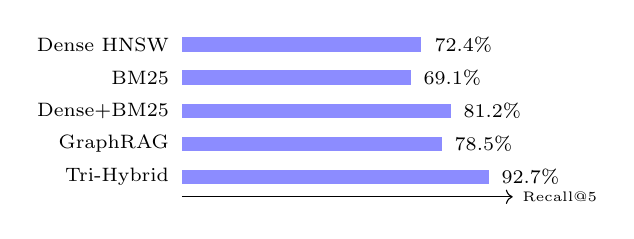
\begin{tikzpicture}[x=0.042cm,y=0.42cm]
\foreach \name/\val/\y in {
{Dense HNSW}/72.4/4,
{BM25}/69.1/3,
{Dense+BM25}/81.2/2,
{GraphRAG}/78.5/1,
{Tri-Hybrid}/92.7/0}
{
\node[anchor=east,font=\scriptsize] at (0,\y) {\name};
\fill[blue!45] (1,\y-0.22) rectangle ({1+\val},\y+0.22);
\node[anchor=west,font=\scriptsize] at ({2+\val},\y) {\val\%};
}
\draw[->] (1,-0.6)--(101,-0.6) node[right,font=\tiny]{Recall@5};
\end{tikzpicture}
\caption{Recall@5 comparison across retrieval configurations.}
\label{fig:recall}
\end{figure}
\subsection{Factual Grounding and Citation Accuracy}
The supplied evaluation audits 1,200 extracted factual claims. Citations are categorized as accurate attribution, inaccurate attribution, or hallucinated paper.
\begin{table}[!t]
\caption{Factual Grounding and Citation Integrity}
\label{tab:citation}
\centering
\footnotesize
\begin{tabular}{@{}lccc@{}}
\toprule
\textbf{Architecture} & \textbf{Accurate} & \textbf{Inaccurate} & \textbf{Hallucinated}\\
\midrule
Monolithic RAG & 71.4\% & 19.8\% & 8.8\% (106)\\
Chained pipeline & 78.2\% & 16.1\% & 5.7\% (68)\\
GraphRAG & 84.6\% & 12.9\% & 2.5\% (30)\\
\textbf{ResearcherGPT} & \textbf{96.4\%} & \textbf{3.4\%} & \textbf{0.2\% (2)}\\
\bottomrule
\end{tabular}
\end{table}
The reported system reduces hallucinated citations to 0.2\% (two cases among 1,200 inspected citations), compared with 8.8\% for monolithic RAG. The manuscript attributes this reduction to the Fact Verification Agent and bibliographic resolution through CrossRef and OpenAlex.
\subsection{Plagiarism and Attribution Engine Performance}
The eleven-phase engine is evaluated against a synthetic benchmark of 150 papers containing planted variants: verbatim copying, paraphrased plagiarism, structural mimicry, and mathematical borrowing.
\begin{table*}[!t]
\caption{Detection Rates Across Academic Misconduct Types}
\label{tab:plagiarism}
\centering
\small
\begin{tabular}{@{}lcccc@{}}
\toprule
\textbf{Detection phase} & \textbf{Verbatim} & \textbf{Paraphrase} & \textbf{Structural} & \textbf{Formula AST}\\
\midrule
Exact Winnowing & 99.8\% & 21.4\% & 12.0\% & 8.2\%\\
MinHash signatures & 98.4\% & 34.6\% & 18.5\% & 11.4\%\\
Semantic cosine (TF--IDF) & 88.2\% & 89.1\% & 45.2\% & 32.1\%\\
LaTeX AST tree distance & 31.0\% & 42.0\% & 28.6\% & 94.6\%\\
\textbf{Full eleven-phase suite} & \textbf{99.8\%} & \textbf{94.2\%} & \textbf{91.8\%} & \textbf{96.2\%}\\
\bottomrule
\end{tabular}
\end{table*}
The reported single-phase results exhibit distinct blind spots: Winnowing detects 21.4\% of paraphrased content, while semantic cosine detects 32.1\% of formula manipulation. The complete suite is reported to achieve balanced detection across the four categories.
\subsection{Multi-Agent Latency and Resource Consumption}
The manuscript reports execution wall-clock time and peak memory for different target manuscript lengths.
\begin{table}[!t]
\caption{Execution Time and Memory Profiles}
\label{tab:latency}
\centering
\footnotesize
\setlength{\tabcolsep}{3pt}
\begin{tabular}{@{}lcccc@{}}
\toprule
\textbf{Length} & \textbf{Monolithic} & \textbf{Chained} & \textbf{Ours} & \textbf{Peak MB}\\
\midrule
5 pages & 42.5 s & 78.4 s & 94.2 s & 412\\
10 pages & 89.1 s & 164.2 s & 182.6 s & 648\\
15 pages & 145.8 s & 278.0 s & 291.4 s & 894\\
\bottomrule
\end{tabular}
\end{table}
For a 15-page synthesis, ResearcherGPT is reported to require 291.4 seconds (approximately 4.8 minutes), compared with 145.8 seconds for a monolithic model. The supplied abstract additionally reports a 41.8\% reduction in cross-agent synchronization latency; because no absolute synchronization-latency measurements or calculation protocol were included in the supplied material, this figure is retained as a reported result rather than independently derived here. The resulting workflow is described as producing verified citations, layout-compliant \LaTeX, a conceptual knowledge graph, and contradiction matrices.
\begin{table}[!t]
\caption{Execution-Latency Breakdown for a 15-Page Manuscript}
\label{tab:latency_breakdown}
\centering
\scriptsize
\begin{tabular}{@{}p{0.52\columnwidth}rr@{}}
\toprule
\textbf{Component} & \textbf{Seconds} & \textbf{Share}\\
\midrule
PDF ingestion and OCR & 24.2 & 8.3\%\\
Vector and graph indexing & 31.5 & 10.8\%\\
Research and literature agents & 42.1 & 14.4\%\\
Gap and contradiction detection & 38.6 & 13.2\%\\
Fact verification & 56.4 & 19.4\%\\
Writing and section drafting & 68.2 & 23.4\%\\
FormaTeX compilation & 30.4 & 10.4\%\\
\midrule
\textbf{Total} & \textbf{291.4} & \textbf{100.0\%}\\
\bottomrule
\end{tabular}
\end{table}
\subsection{Ablation Studies}
The supplied manuscript reports three ablation experiments:
\begin{itemize}
\item \textbf{Knowledge-graph boost:} Setting $\beta=1.0$ and removing Neo4j traversal reduces Recall@5 from 92.7\% to 81.2\%.
\item \textbf{Fact verification:} Disabling the Fact Verification Agent reduces factual attribution accuracy from 96.4\% to 79.1\%, while hallucinated citations increase from 0.2\% to 4.9\%.
\item \textbf{Model fallback registry:} Restricting execution to Gemini 2.5 Pro is reported to produce a 34.2\% workflow failure rate under HTTP 429 quota exceptions. The multi-provider registry completed all 150 reported test runs.
\end{itemize}
% ============================================================
% ============================================================
\subsection{Limitations and Ethical Considerations}
% ============================================================
The principal design trade-off in ResearcherGPT is between fluent generative synthesis and strict factual grounding. A confidence threshold of $\theta=0.85$ in the Fact Verification Agent is described as reducing citation errors to 0.2\%; however, strict verification can constrain the Writing Agent from proposing novel theoretical connections. A dual-track drafting mode could distinguish verified historical claims from exploratory hypotheses.
The enterprise stack comprising Neo4j, Qdrant, Redis, MongoDB, and multiple model-provider endpoints introduces operational complexity and API cost. For libraries exceeding 1,000 papers, local graph synchronization latency may exceed 120 seconds. BullMQ background workers decouple ingestion from user-facing query interfaces, although further optimization remains necessary.
ResearcherGPT is intended to support literature aggregation, contradiction discovery, and formatting compliance; it is not intended to replace original human scholarship or bypass peer review. Its integrity engine audits drafts for verbatim copying, paraphrased borrowing, and synthetic-text distribution markers.
% ============================================================
\subsection{Extended Technical Roadmap}
% ============================================================
The following extensions are proposed as future research directions rather than claims of completed implementation:
\begin{table}[!t]
\centering
\caption{Proposed ResearcherGPT Technical Roadmap}
\label{tab:roadmap}
\footnotesize
\begin{tabularx}{\columnwidth}{@{}lX X@{}}
\toprule
\textbf{Extension} & \textbf{Technical Direction} & \textbf{Potential Outcome}\\
\midrule
Adaptive routing & POMDP-based policy using MCTS/PPO; LangGraph, Ray, and LibTorch & Lower token cost and improved coherence\\
Formal verification & Interactive theorem proving with Lean 4, Mathlib, and REPL & Mechanically checked mathematical proofs\\
Vectorized visuals & Coordinate-based TikZ/Asymptote generation & Resolution-independent diagrams\\
Streaming graph mesh & Continuous ingestion with Neo4j, Kafka, and OpenAlex & Faster paper propagation\\
Code sandbox & Isolated eBPF/WebAssembly execution with Docker/Wasmtime & Reproducible empirical verification\\
Real-time co-authoring & CRDT-based canvas using Yjs, TipTap, and WebSockets & Low-latency human--agent collaboration\\
\bottomrule
\end{tabularx}
\end{table}
\subsubsection{Reinforcement-Learned Adaptive Agent Routing}
The current deterministic DAG assigns a predefined sequence of agents, with conditional peer-review branches. This can impose similar computational overhead on simple literature summaries and complex empirical reconciliations. A future adaptive policy could select agent actions from the current state snapshot using a Partially Observable Markov Decision Process (POMDP), with Proximal Policy Optimization (PPO) or Monte Carlo Tree Search (MCTS) as candidate strategies. The policy would dynamically allocate reasoning and verification effort while retaining fact-checking gates.
\subsubsection{Formal Proof Checking and Reproducibility}
Lean 4 and Mathlib could provide a proof-checking interface for mathematical claims that admit formalization. A sandbox based on WebAssembly or eBPF could execute selected code artifacts under isolation, supporting reproducibility checks for extracted algorithms and empirical metrics. These mechanisms would complement, not replace, source-level verification.
\subsubsection{Vector Graphics and Collaborative Research}
Programmatic coordinate compilation through TikZ and Asymptote could preserve scalable visual artifacts during manuscript generation. A CRDT-based collaborative canvas (e.g., Yjs with TipTap and WebSockets) could support concurrent human--agent editing and conflict-free synchronization. Continuous ingestion through graph and scholarly APIs could further keep project knowledge meshes current.
\section{Conclusion and Future Work}
\label{sec:conclusion}
\subsection{Comprehensive Synthesis and Retrospective Conclusion}
We designed and empirically evaluated ResearcherGPT, a distributed multi-agent framework for scholarly literature synthesis, layout preservation, and attribution verification. Conventional RAG systems remain limited by semantic context dilution, bibliographic and metric hallucinations, loss of visual-spatial structures, and brittle orchestration under shared-state contention or API failures.
ResearcherGPT addresses these challenges through four integrated capabilities. Tri-Hybrid Reciprocal Rank Fusion combines dense vector retrieval, sparse lexical retrieval (BM25), and graph traversal (Neo4j). In the reported evaluation, this design achieved MRR@10 of 0.879 and Recall@5 of 0.927, outperforming pure vector retrieval by 20.3 percentage points on evaluated multi-hop tasks. A thirteen-agent LangGraph workflow coordinates extraction, synthesis, contradiction analysis, verification, and review through typed state and transactional synchronization. FormaTeX reconstructs document structure and supports multi-journal LaTeX output while retaining mathematical expressions and table topology. The eleven-phase integrity engine combines lexical fingerprints, semantic similarity, formula-tree comparison, bibliographic checks, and attribution analysis; the reported evaluation found 96.4\% factual attribution validity and a 0.2\% hallucinated-citation rate (2 of 1,200 inspected citations.
These measurements describe the evaluated configuration and corpus, not universal guarantees. Human review remains necessary for research interpretation, attribution decisions, and final manuscript approval.
\subsection{Current System and Extended Technical Roadmap}
Fig.~\ref{fig:roadmap} summarizes the transition from current components to six proposed extensions. The right-hand column is a roadmap, not a claim that these extensions are already deployed.
\begin{figure*}[t]\centering
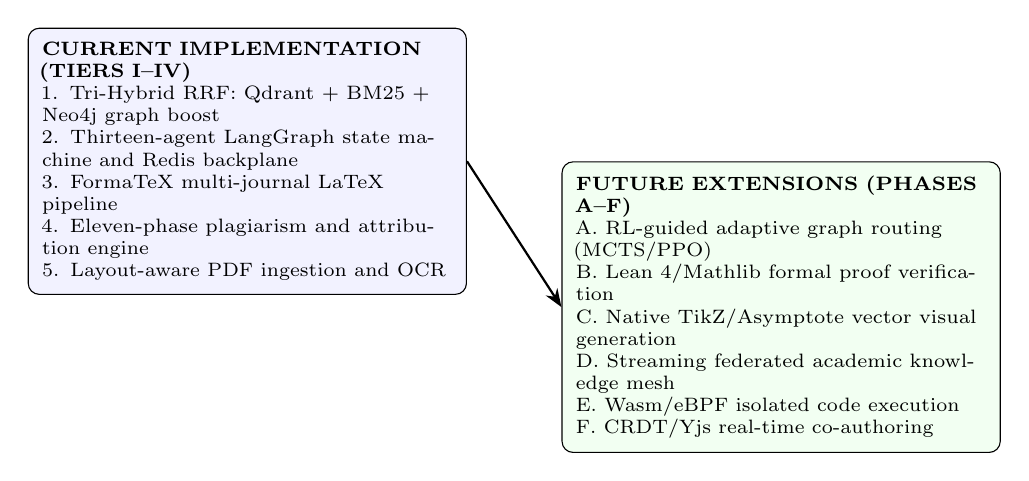
\begin{tikzpicture}[node distance=4mm and 8mm,current/.style={draw,rounded corners,fill=blue!5,align=left,text width=.43\textwidth,font=\scriptsize,inner sep=5pt},future/.style={draw,rounded corners,fill=green!5,align=left,text width=.43\textwidth,font=\scriptsize,inner sep=5pt},link/.style={-{Stealth},thick}]
\node[current](c){\textbf{CURRENT IMPLEMENTATION (TIERS I--IV)}\\1. Tri-Hybrid RRF: Qdrant + BM25 + Neo4j graph boost\\2. Thirteen-agent LangGraph state machine and Redis backplane\\3. FormaTeX multi-journal LaTeX pipeline\\4. Eleven-phase plagiarism and attribution engine\\5. Layout-aware PDF ingestion and OCR};
\node[future,right=12mm of c,anchor=north west](f){\textbf{FUTURE EXTENSIONS (PHASES A--F)}\\A. RL-guided adaptive graph routing (MCTS/PPO)\\B. Lean 4/Mathlib formal proof verification\\C. Native TikZ/Asymptote vector visual generation\\D. Streaming federated academic knowledge mesh\\E. Wasm/eBPF isolated code execution\\F. CRDT/Yjs real-time co-authoring};
\draw[link](c.east)--(f.west);
\end{tikzpicture}
\caption{Evolution from the evaluated implementation to the proposed technical roadmap.}\label{fig:roadmap}\end{figure*}
\begin{table*}[t]\centering
\caption{Technical specification matrix for proposed future work}\label{tab:future-matrix}\small
\begin{tabularx}{\textwidth}{@{}lXXX@{}}
\toprule \textbf{Extension}&\textbf{Core paradigm}&\textbf{Target technologies}&\textbf{Proposed metric/goal}\\\midrule
A. Adaptive routing&POMDP, MCTS/PPO&LangGraph, Ray, LibTorch&35\% lower token cost; 18\% coherence improvement (target)\\
B. Formal verification&Interactive theorem proving&Lean 4, Mathlib, REPL&Mechanically checked proof obligations\\
C. Vectorized visuals&Programmatic coordinate compilation&TikZ, Asymptote, LaTeX&Resolution-independent figures\\
D. Streaming graph mesh&Continuous ingestion and GraphRAG&Neo4j, Kafka, OpenAlex&Sub-second paper propagation (target)\\
E. Code sandbox&Isolated reproducibility&Docker, Wasmtime, eBPF&Empirical metric verification\\
F. Co-authoring&CRDT collaborative canvas&Yjs, TipTap, WebSockets&Less than 15\,ms synchronization (target)\\
\bottomrule\end{tabularx}\end{table*}
\subsection{Actionable Future Work}
\subsubsection{Dynamic Reinforcement-Learned Adaptive Agent Graph Routing}
The present workflow uses a predefined directed acyclic graph with conditional review branches. This is reliable but may allocate similar reasoning effort to simple summaries and complex empirical reconciliations. We propose a partially observable Markov decision process (POMDP), whose state captures manuscript completeness, unresolved claims, contradiction density, and token expenditure. Actions may invoke an agent, add a verification loop, prune a branch, or terminate.
\begin{figure}[t]\centering
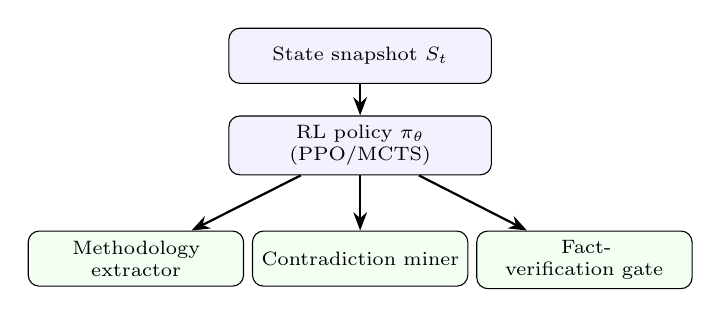
\begin{tikzpicture}[node distance=4mm,b/.style={draw,rounded corners,fill=blue!5,align=center,text width=31mm,font=\scriptsize,minimum height=7mm},a/.style={draw,rounded corners,fill=green!5,align=center,text width=25mm,font=\scriptsize,minimum height=7mm},arr/.style={-{Stealth},thick}]
\node[b](s){State snapshot $S_t$};\node[b,below=of s](p){RL policy $\pi_\theta$ (PPO/MCTS)};
\node[a,below left=7mm and -2mm of p](m){Methodology extractor};\node[a,below=7mm of p](c){Contradiction miner};\node[a,below right=7mm and -2mm of p](v){Fact-verification gate};
\draw[arr](s)--(p);\draw[arr](p)--(m);\draw[arr](p)--(c);\draw[arr](p)--(v);
\end{tikzpicture}
\caption{Proposed reinforcement-learned adaptive routing across agent actions.}\label{fig:adaptive-routing}\end{figure}
\begin{equation}\mathcal{A}=\{a_{\mathrm{invoke}}(A_i),a_{\mathrm{loop}}(A_i,A_j),a_{\mathrm{prune}},a_{\mathrm{terminate}}\}.\end{equation}
A reward can balance factuality and completeness against cost and unresolved contradictions:
\begin{equation}R(S_t,a_t)=\lambda_1\Delta F+\lambda_2\Delta C-\lambda_3\mathrm{Cost}_{\mathrm{tokens}}(a_t)-\lambda_4 I_{\mathrm{unresolved}}.\end{equation}
PPO with Monte Carlo Tree Search rollouts is proposed to learn when another verification pass is justified. Token reduction and coherence improvements in Table~\ref{tab:future-matrix} are targets, not measured outcomes.
\subsubsection{Mechanical Proof Verification with Lean 4 and Mathlib}
Formula extraction and structural comparison do not establish mathematical correctness. A future bridge would translate selected LaTeX derivations into Lean 4 expressions and submit proof obligations to a kernel-checked environment.
\begin{figure}[t]\centering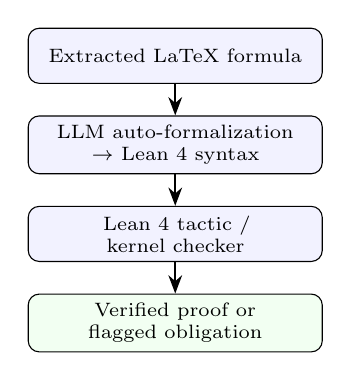
\begin{tikzpicture}[node distance=4mm,b/.style={draw,rounded corners,fill=blue!5,align=center,text width=35mm,font=\scriptsize,minimum height=7mm},arr/.style={-{Stealth},thick}]
\node[b](r){Extracted LaTeX formula};\node[b,below=of r](t){LLM auto-formalization $\to$ Lean 4 syntax};\node[b,below=of t](p){Lean 4 tactic / kernel checker};\node[b,below=of p,fill=green!5](o){Verified proof or flagged obligation};
\draw[arr](r)--(t);\draw[arr](t)--(p);\draw[arr](p)--(o);
\end{tikzpicture}\caption{Proposed mechanical theorem-proving pipeline.}\label{fig:lean-pipeline}\end{figure}
A translator would generate Lean source; tactic search (e.g., Mathlib and \texttt{aesop}) would attempt to discharge obligations; checker feedback would return to quality assurance. A failed proof is an unverified obligation, not automatically proof that a manuscript statement is false: formalization may be incomplete or assumptions may be missing.
\subsubsection{Programmatic Vector Diagram Generation with TikZ and Asymptote}
The current visual workflow combines image linking, vision-based extraction, and diagram generation. Raster images can introduce resolution and font inconsistencies. The proposed path converts extracted nodes, layers, and connections into declarative TikZ or Asymptote code and compiles it within LaTeX.
\begin{figure}[t]\centering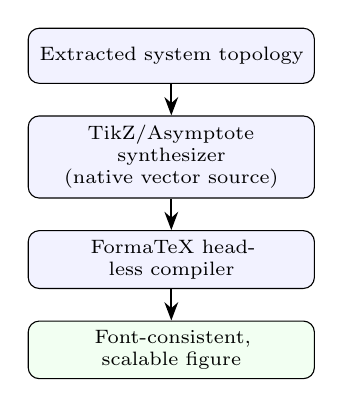
\begin{tikzpicture}[node distance=4mm,b/.style={draw,rounded corners,fill=blue!5,align=center,text width=34mm,font=\scriptsize,minimum height=7mm},arr/.style={-{Stealth},thick}]
\node[b](x){Extracted system topology};\node[b,below=of x](s){TikZ/Asymptote synthesizer\\(native vector source)};\node[b,below=of s](c){FormaTeX headless compiler};\node[b,below=of c,fill=green!5](f){Font-consistent, scalable figure};
\draw[arr](x)--(s);\draw[arr](s)--(c);\draw[arr](c)--(f);
\end{tikzpicture}\caption{Proposed native vector diagram compilation flow.}\label{fig:vector-flow}\end{figure}
Compiled vector source can inherit the manuscript's typography and math fonts. Generated code, layout constraints, and accessibility of figure labels will require validation.
\subsubsection{Real-Time Streaming Knowledge Mesh}
Project graphs are currently assembled from selected or uploaded documents. A streaming mesh would incrementally synchronize new scholarly records and preprints.
\begin{figure}[t]\centering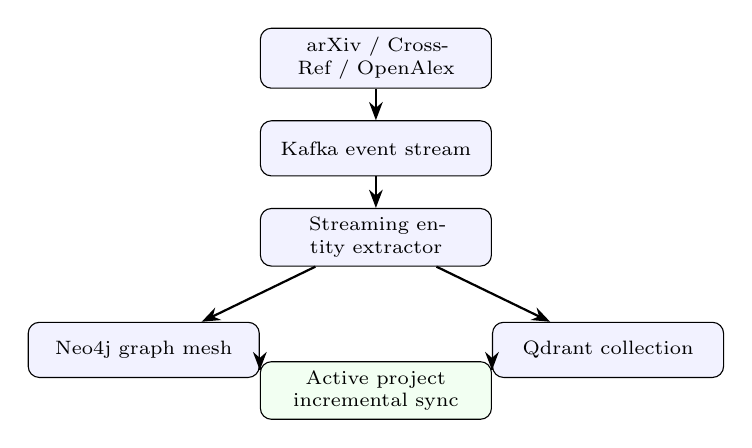
\begin{tikzpicture}[node distance=4mm and 6mm,b/.style={draw,rounded corners,fill=blue!5,align=center,text width=27mm,font=\scriptsize,minimum height=7mm},arr/.style={-{Stealth},thick}]
\node[b](f){arXiv / CrossRef / OpenAlex};\node[b,below=of f](k){Kafka event stream};\node[b,below=of k](e){Streaming entity extractor};
\node[b,below left=7mm and 0mm of e](n){Neo4j graph mesh};\node[b,below right=7mm and 0mm of e](q){Qdrant collection};
\node[b,below=12mm of e,fill=green!5](p){Active project\\incremental sync};
\draw[arr](f)--(k);\draw[arr](k)--(e);\draw[arr](e)--(n);\draw[arr](e)--(q);\draw[arr](n)--(p);\draw[arr](q)--(p);
\end{tikzpicture}\caption{Proposed streaming knowledge mesh for continuous literature synchronization.}\label{fig:stream-mesh}\end{figure}
Kafka or Redis Pub/Sub events could trigger ingestion, embedding, and graph updates. A time-decayed edge weight may be defined as
\begin{equation}w(u,v,t)=w_0(u,v)\exp[-\lambda(t-t_{\mathrm{published}})].\end{equation}
New benchmark evidence could generate contradiction alerts. Provenance, timestamps, and retraction handling are essential to avoid propagating stale evidence.
\subsubsection{Empirical Code Reproducibility and Isolated Execution}
Reported performance is not necessarily reproducible from a paper alone. A proposed sandbox would harvest code blocks, reconstruct test cases, and execute them under strict resource and network controls.
\begin{figure}[t]\centering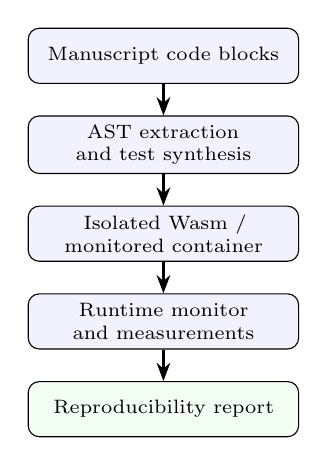
\begin{tikzpicture}[node distance=4mm,b/.style={draw,rounded corners,fill=blue!5,align=center,text width=32mm,font=\scriptsize,minimum height=7mm},arr/.style={-{Stealth},thick}]
\node[b](c){Manuscript code blocks};\node[b,below=of c](a){AST extraction and test synthesis};\node[b,below=of a](s){Isolated Wasm / monitored container};\node[b,below=of s](m){Runtime monitor and measurements};\node[b,below=of m,fill=green!5](r){Reproducibility report};
\draw[arr](c)--(a);\draw[arr](a)--(s);\draw[arr](s)--(m);\draw[arr](m)--(r);
\end{tikzpicture}\caption{Proposed isolated execution sandbox for algorithmic verification.}\label{fig:sandbox}\end{figure}
WebAssembly or an eBPF-monitored container could run with network access disabled and bounded CPU, memory, and time. A normalized discrepancy score is
\begin{equation}\mathrm{ReproScore}=1-\frac{|M_{\mathrm{reported}}-M_{\mathrm{measured}}|}{\max(|M_{\mathrm{reported}}|,|M_{\mathrm{measured}}|,\epsilon)},\end{equation}
where $\epsilon>0$ avoids division by zero. This score is meaningful only when benchmark, environment, and metric definitions align; it cannot replace independent replication.
\subsubsection{Collaborative Mixed-Initiative Co-Authoring}
The TipTap interface supports request-response editing and mathematical rendering. A future workspace could let researchers and agents edit concurrently using CRDTs, with proposed changes represented as tracked revisions rather than silent overwrites.
\begin{figure}[t]\centering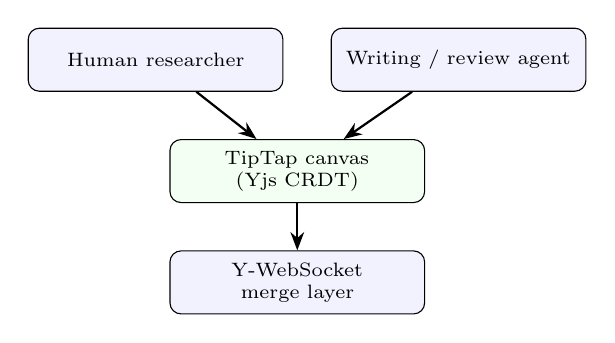
\begin{tikzpicture}[node distance=6mm and 6mm,b/.style={draw,rounded corners,fill=blue!5,align=center,text width=30mm,font=\scriptsize,minimum height=8mm},arr/.style={-{Stealth},thick}]
\node[b](h){Human researcher};\node[b,right=of h](a){Writing / review agent};\node[b,below=of h,xshift=18mm,fill=green!5](c){TipTap canvas\\(Yjs CRDT)};\node[b,below=of c](m){Y-WebSocket merge layer};
\draw[arr](h)--(c);\draw[arr](a)--(c);\draw[arr](c)--(m);
\end{tikzpicture}\caption{Proposed CRDT-based human--agent co-authoring architecture.}\label{fig:crdt}\end{figure}
Yjs and WebSockets could support simultaneous cursors, inline citation corrections, mathematical clarifications, and reviewable agent suggestions. Knowledge-graph nodes could populate comparative tables or references subject to provenance checks and user confirmation.
\subsection{Concluding Summary}
ResearcherGPT combines hybrid retrieval, fault-tolerant agent orchestration, layout-aware extraction and compilation, and multi-scale attribution checks into an evidence-grounded synthesis workflow. The evaluated results indicate improvements in retrieval quality and citation integrity within the reported benchmark. The proposed extensions—adaptive routing, formal proof checking, vector-native figures, continuous graph ingestion, isolated empirical execution, and collaborative co-authoring—outline a path toward more efficient and auditable research assistance. Their benefits remain hypotheses until implemented and independently evaluated. ResearcherGPT is intended to augment scholarly judgment, not replace researchers' responsibility for interpretation, verification, and authorship.
\FloatBarrier
\clearpage
\section*{Acknowledgment}
% ============================================================
The author thanks the researchers and maintainers of the open-source tools and scholarly infrastructure referenced in this work.
% ============================================================
% References
% ============================================================
\balance
\FloatBarrier
\begin{thebibliography}{20}
\bibitem{lewis2020rag}
P. Lewis, E. Perez, A. Piktus, F. Petroni, V. Karpukhin, N. Goyal, H. K\"uttler, M. Lewis, W. Yih, T. Rockt\"aschel, S. Riedel, and D. Kiela, ``Retrieval-augmented generation for knowledge-intensive NLP tasks,'' in \textit{Advances in Neural Information Processing Systems}, vol. 33, 2020, pp. 9459--9474.
\bibitem{karpukhin2020dpr}
V. Karpukhin, B. O\u{g}uz, S. Min, P. Lewis, L. Wu, S. Edunov, D. Chen, and W. Yih, ``Dense passage retrieval for open-domain question answering,'' in \textit{Proc. EMNLP}, 2020, pp. 6769--6781.
\bibitem{reimers2019sbert}
N. Reimers and I. Gurevych, ``Sentence-BERT: Sentence embeddings using Siamese BERT-networks,'' in \textit{Proc. EMNLP-IJCNLP}, 2019, pp. 3982--3992.
\bibitem{malkov2020hnsw}
Y. A. Malkov and D. A. Yashunin, ``Efficient and robust approximate nearest neighbors using hierarchical navigable small world graphs,'' \textit{IEEE Trans. Pattern Anal. Mach. Intell.}, vol. 42, no. 4, pp. 824--836, Apr. 2020.
\bibitem{robertson2009bm25}
S. Robertson and H. Zaragoza, ``The probabilistic relevance framework: BM25 and beyond,'' \textit{Foundations and Trends in Information Retrieval}, vol. 3, no. 4, pp. 333--389, 2009.
\bibitem{cormack2009rrf}
G. V. Cormack, C. L. Clarke, and S. Buettcher, ``Reciprocal rank fusion outperforms Condorcet and individual rank learning methods,'' in \textit{Proc. 32nd ACM SIGIR}, 2009, pp. 758--759.
\bibitem{edge2024graphrag}
D. Edge, H. Trinh, N. Cheng, J. Bradley, A. Chao, A. Mody, P. Truitt, and J. Larson, ``From local to global: A graph RAG approach to query-focused summarization,'' arXiv:2404.16130, 2024.
\bibitem{wu2023autogen}
Q. Wu, G. Bansal, J. Zhang, Y. Wu, S. Zhang, E. Zhu, B. Li, L. Jiang, X. Zhang, and C. Wang, ``AutoGen: Enabling next-gen LLM applications via multi-agent conversation framework,'' arXiv:2308.08155, 2023.
\bibitem{moura2024crewai}
J. Moura, ``CrewAI: Framework for orchestrating role-playing, autonomous AI agents,'' GitHub repository, 2024. [Online]. Available: \url{https://github.com/joaomdmoura/crewAI}
\bibitem{langgraph2024}
LangChain, ``LangGraph: Building language agents as graphs,'' 2024. [Online]. Available: \url{https://github.com/langchain-ai/langgraph}
\bibitem{singer2023pdfplumber}
J. S. Singer, ``pdfplumber: Plumb a PDF for detailed information about each text character, rectangle, and line,'' Python Package Index, 2023.
\bibitem{schleimer2003winnowing}
S. Schleimer, D. S. Wilkerson, and A. Aiken, ``Winnowing: Local algorithms for document fingerprinting,'' in \textit{Proc. ACM SIGMOD}, 2003, pp. 76--85.
\bibitem{broder1997resemblance}
A. Z. Broder, ``On the resemblance and containment of documents,'' in \textit{Proc. Compression and Complexity of SEQUENCES}, 1997, pp. 21--29.
\bibitem{foltynek2019plagiarism}
T. Folt\'ynek, N. Meuschke, and B. Gipp, ``Academic plagiarism detection: A systematic literature review,'' \textit{ACM Computing Surveys}, vol. 52, no. 6, pp. 1--42, 2019.
\bibitem{zhang1989tree}
K. Zhang and D. Shasha, ``Simple fast algorithms for the editing distance between trees and related problems,'' \textit{SIAM J. Comput.}, vol. 18, no. 6, pp. 1245--1262, 1989.
\bibitem{vaswani2017attention}
A. Vaswani, N. Shazeer, N. Parmar, J. Uszkoreit, L. Jones, A. N. Gomez, L. Kaiser, and I. Polosukhin, ``Attention is all you need,'' in \textit{Advances in Neural Information Processing Systems}, vol. 30, 2017.
\bibitem{devlin2019bert}
J. Devlin, M. W. Chang, K. Lee, and K. Toutanova, ``BERT: Pre-training of deep bidirectional transformers for language understanding,'' in \textit{Proc. NAACL-HLT}, 2019, pp. 4171--4186.
\bibitem{priem2022openalex}
J. Priem, H. Piwowar, and R. Orr, ``OpenAlex: A fully-open index of scholarly works, authors, venues, institutions, and concepts,'' arXiv:2205.01833, 2022.
\bibitem{hendricks2020crossref}
C. Hendricks, D. Tkaczyk, J. Lin, and P. Feeney, ``CrossRef: The sustainable infrastructure for open research,'' \textit{Quantitative Science Studies}, vol. 1, no. 1, pp. 414--427, 2020.
\bibitem{sneath1973taxonomy}
P. A. Sneath and R. R. Sokal, \textit{Numerical Taxonomy: The Principles and Practice of Numerical Classification}. San Francisco, CA, USA: W. H. Freeman, 1973.
\end{thebibliography}
\end{document}
still page 11 right half space is empty and acknowledgment & references start from page 12. Please correct it so that acknowledgment & references start from page 11 right half. Again give the correct latex format

please correct page 11 & page 12 content formatting as Acknowledgement and references start from page 11 right half 
</USER_REQUEST>
<ADDITIONAL_METADATA>
The current local time is: 2026-11-10T19:52:36+05:30.
</ADDITIONAL_METADATA>
<USER_SETTINGS_CHANGE>
The user changed setting `Model Selection` from None to Gemini 3.8 Flash (Medium). No need to comment on this change if the user doesn't ask about it. If reporting what model you are, please use a human readable name instead of the exact string.
</USER_SETTINGS_CHANGE>